\section{Maloya: langage dédié aux services sensibles au contexte}


\begin{frame}{Une approche dédiée à l'assistance domiciliaire}
\begin{figure}
  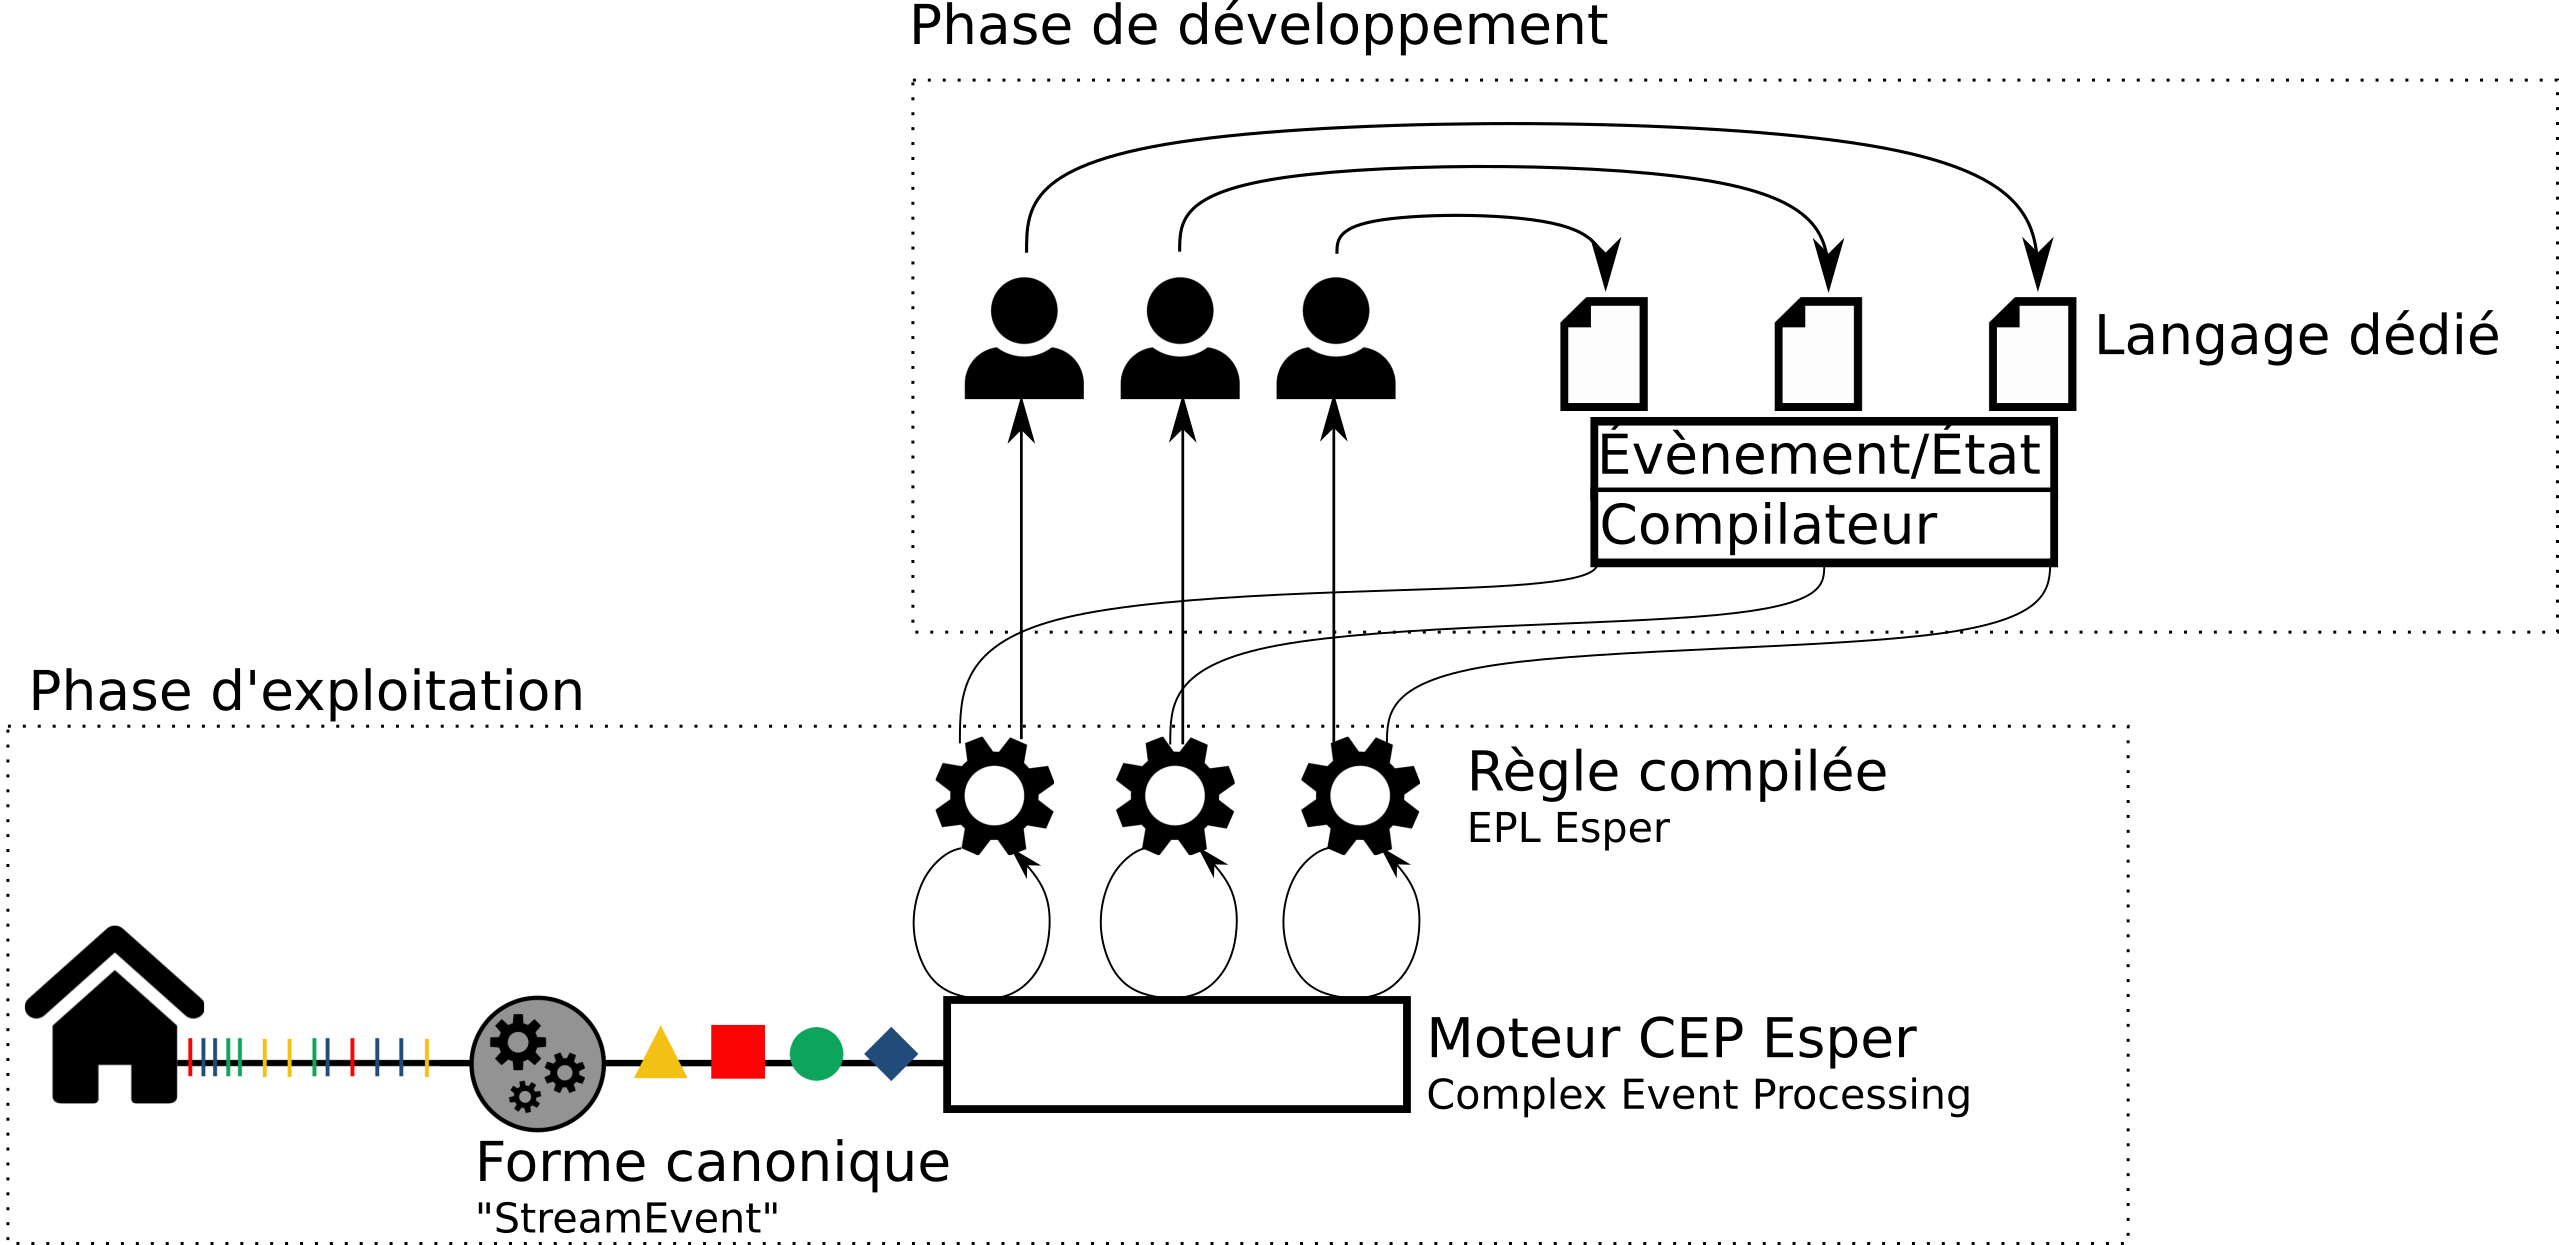
\includegraphics[scale=0.2]{approach_1.png}
\end{figure}
\end{frame}
\begin{frame}{Une approche dédiée à l'assistance domiciliaire}
\addtocounter{framenumber}{-1}
\begin{figure}
  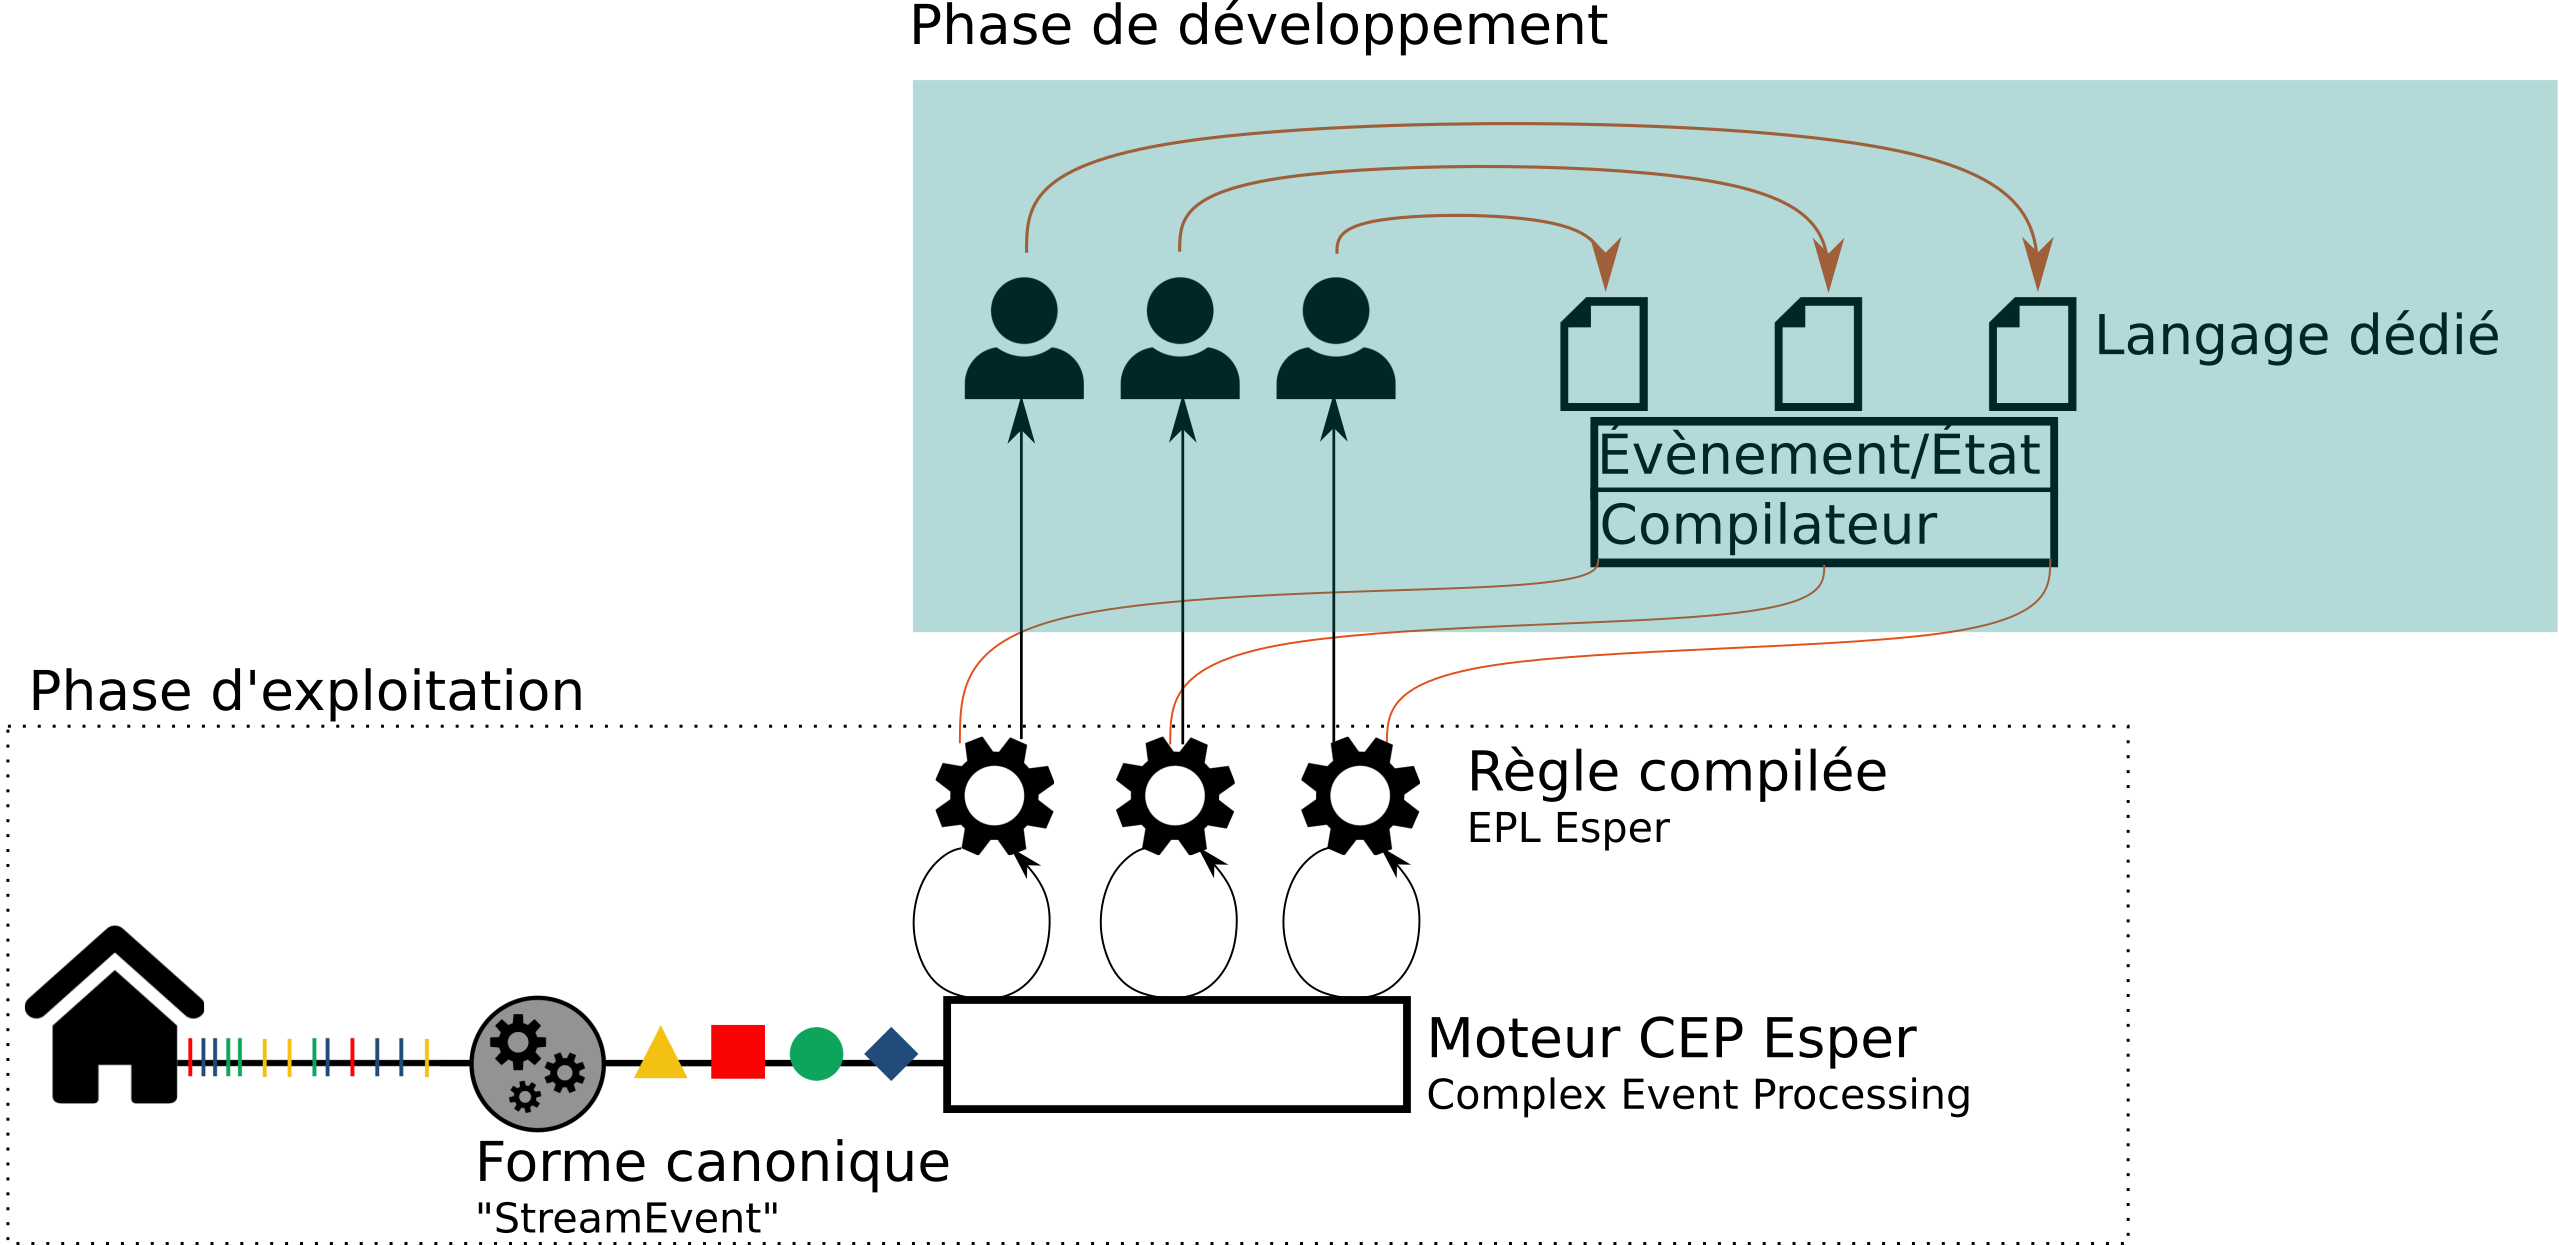
\includegraphics[scale=0.2]{approach_2.png}
\end{figure}
\end{frame}
\begin{frame}{Une approche dédiée à l'assistance domiciliaire}
\addtocounter{framenumber}{-1}
\begin{figure}
  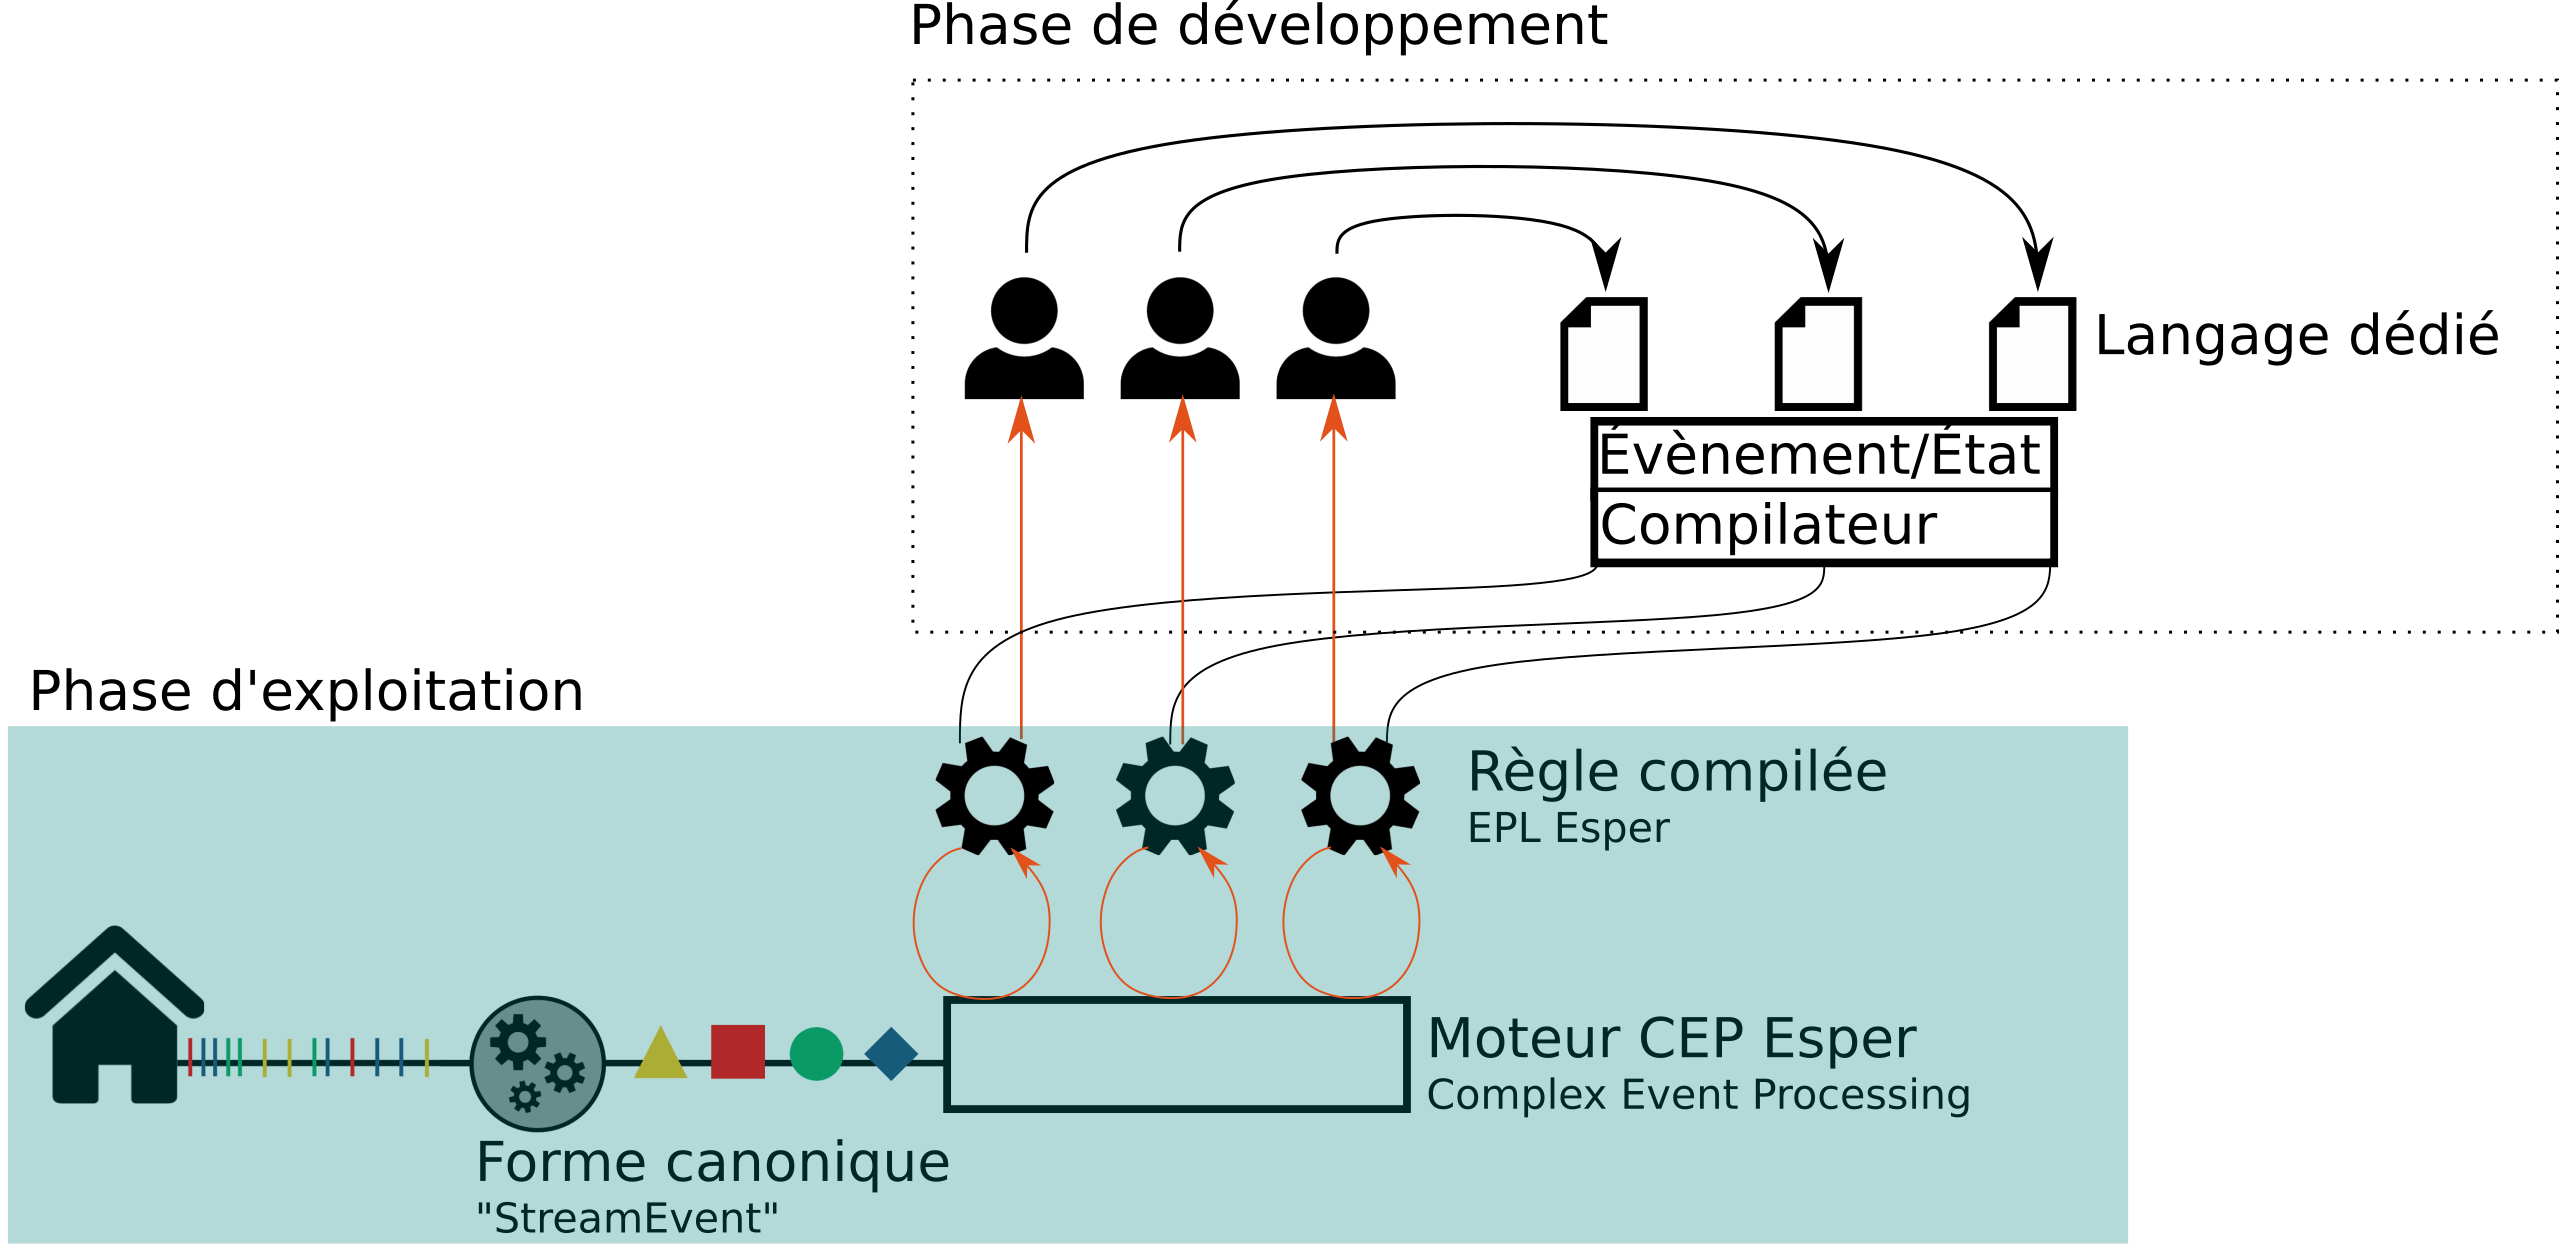
\includegraphics[scale=0.2]{approach_3.png}
\end{figure}
\end{frame}

% \begin{frame}{Scénarios d'assistance domiciliaire}
%   \begin{minipage}[t]{0.45\linewidth}
%     \begin{table}[!h]
%       \begin{footnotesize}
%         \begin{tabular}{| p{2.cm} | p{5.5cm} |} \hline
%           {\bf Nom} & {\bf Description} \\ \hline \hline
%           %Alerte porte d'entrée & Entrance door \colorbox{blue!5}{is open} \colorbox{teal!10}{and}  \colorbox{blue!5}{is unattended} \colorbox{teal!10}{for 5 minutes} \\ \hline
%           Réchauffer un plat surgelé  & Freezer \colorbox{checked!10}{gets used} and stove \colorbox{checked!10}{gets turned on} \colorbox{teal!10}{within 10 minutes} \colorbox{teal!10}{or} Freezer \colorbox{checked!10}{gets used} \colorbox{teal!10}{during} stove \colorbox{blue!5}{is on}, \colorbox{teal!10}{during} \colorbox{blue!5}{lunch time} \\ \hline
%           %Dépendance de présence & The cupboard \colorbox{checked!10}{gets opened} in the kitchen, \colorbox{teal!10}{while} a presence in the kitchen \colorbox{blue!5}{is false} \\ \hline
%           %Échec de communication & A sensor \colorbox{blue!5}{fails to communicate} \colorbox{teal!10}{for 24 hours} %and its status does not \dashuline{get updated} 
%           %\\ \hline
%         \end{tabular}
%       \end{footnotesize}
%     \end{table}
%   \end{minipage}
%   \hfill
%   \begin{minipage}[t]{0.38\linewidth}
%     Commonalités:
%     \begin{itemize}
%     \item Mesures d'environnement (physique et numérique).
%     \item \colorbox{checked!10}{Évènements}.
%     \item \colorbox{blue!5}{États}.
%     \end{itemize}
%     Variabilités:
%     \begin{itemize}
%     \item Niveaux d'abstraction.
%     \item \colorbox{teal!10}{Contraintes d'interactions} (précédence, chevauchement, durée,$~\dots$).
%     \end{itemize}
%   \end{minipage}
% \end{frame}

% \begin{frame}{Scénarios d'assistance domiciliaire}
%   \addtocounter{framenumber}{-1}
%   \begin{minipage}[t]{0.45\linewidth}
%     \begin{table}[!h]
%       \begin{footnotesize}
%         \begin{tabular}{| p{2.cm} | p{5.5cm} |} \hline
%           {\bf Name} & {\bf Description} \\ \hline \hline
%           %Alerte porte d'entrée & Entrance door \colorbox{blue!5}{is open} \colorbox{teal!10}{and}  \colorbox{blue!5}{is unattended} \colorbox{teal!10}{for 5 minutes} \\ \hline
%           \cellcolor{red!10}{Réchauffer un plat surgelé}  & \cellcolor{red!10}{Freezer \colorbox{red!10}{gets used} and stove \colorbox{red!10}{gets turned on} \colorbox{red!10}{within 10 minutes} \colorbox{red!10}{or} Freezer \colorbox{red!10}{gets used} \colorbox{red!10}{during} stove \colorbox{red!10}{is on}, \colorbox{red!10}{during} \colorbox{red!10}{lunch time}} \\ \hline
%           %Dépendance de présence & The cupboard \colorbox{checked!10}{gets opened} in the kitchen, \colorbox{teal!10}{while} a presence in the kitchen \colorbox{blue!5}{is false} \\ \hline
%           %Échec de communication & A sensor \colorbox{blue!5}{fails to communicate} \colorbox{teal!10}{for 24 hours} %and its status does not \dashuline{get updated} 
%           \\ \hline
%         \end{tabular}
%       \end{footnotesize}
%     \end{table}
%   \end{minipage}
%   \hfill
%   \begin{minipage}[t]{0.38\linewidth}
%     Commonalités:
%     \begin{itemize}
%     \item Mesures d'environnement (physique et numérique).
%     \item \colorbox{checked!10}{Évènements}.
%     \item \colorbox{blue!5}{États}.
%     \end{itemize}
%     Variabilités:
%     \begin{itemize}
%     \item Niveaux d'abstraction.
%     \item \colorbox{teal!10}{Contraintes d'interactions} (précédence, chevauchement, durée,$~\dots$).
%     \end{itemize}
%   \end{minipage}
% \end{frame}

\begin{frame}[fragile]{Langage de règles}
  \vspace*{-9.65mm}
  \begin{coloredbox}[gray]{}
    \begin{footnotesize}
      Freezer \colorbox{black!2}{gets opened} \colorbox{black!2}{and} stove gets turned on \colorbox{black!2}{within 10 minutes} or \\Freezer gets opened during stove \colorbox{black!2}{is on}, during lunch time
    \end{footnotesize}
  \end{coloredbox}
  \vfill
  \begin{minipage}{.31\linewidth}
  \end{minipage}
  \hfill
  \begin{minipage}{.31\linewidth} 
  \end{minipage}
  \hfill
  \begin{minipage}{.33\linewidth} 
    \begin{center}
    \end{center}
  \end{minipage}
\end{frame}

\begin{frame}[fragile]{Langage de règles}
  \addtocounter{framenumber}{-1}
  % \vspace*{-3mm}
  \begin{coloredbox}[gray]{}
    \begin{footnotesize}
      Freezer \colorbox{checked!50}{gets opened} \colorbox{black!2}{and} stove gets turned on \colorbox{black!2}{within 10 minutes} or \\Freezer gets opened during stove \colorbox{black!2}{is on}, during lunch time
    \end{footnotesize}
  \end{coloredbox}
  \vfill
  \begin{minipage}{.31\linewidth}
    \begin{coloredbox}[checked]{Évènement~:}
      \begin{lstlisting}[language=MaloyaText]
        //Syntaxe textuelle:
        freezer becomes open
      \end{lstlisting}
      % \begin{lstlisting}[language=Maloya]
      %   //Syntaxe abstraite:
      %   freezer => open
      % \end{lstlisting}
    \end{coloredbox}
  \end{minipage}
  \hfill
  \begin{minipage}{.31\linewidth} 
  \end{minipage}
  \hfill
  \begin{minipage}{.33\linewidth} 
    \begin{center}
    \end{center}
  \end{minipage}
\end{frame}

\begin{frame}[fragile]{Langage de règles}
\addtocounter{framenumber}{-1}
%\vspace*{-3.mm}
  \begin{coloredbox}[gray]{}
    \begin{footnotesize}
      Freezer \colorbox{checked!50}{gets opened} \colorbox{black!2}{and} stove gets turned on \colorbox{black!2}{within 10 minutes} or\\ Freezer gets opened during stove \colorbox{darkgray!50}{is on}, during lunch time
    \end{footnotesize}
  \end{coloredbox}
\vfill
  \begin{minipage}{.31\linewidth}
    \begin{coloredbox}[checked]{Évènement~:}
      \begin{lstlisting}[language=MaloyaText]
        //Syntaxe textuelle:
        freezer becomes open
      \end{lstlisting}
      % \begin{lstlisting}[language=Maloya]
      %   //Syntaxe abstraite:
      %   freezer => open
      % \end{lstlisting}
    \end{coloredbox}
  \end{minipage}
  \hfill
  \begin{minipage}{.31\linewidth}
    \begin{coloredbox}[darkgray]{État~:}
      \begin{lstlisting}[language=MaloyaText]
        //Syntaxe textuelle:
        stove is on
      \end{lstlisting}
      % \begin{lstlisting}[language=Maloya]
      %   //Syntaxe abstraite:
      %   stove = on
      % \end{lstlisting}
    \end{coloredbox}
  \end{minipage}
  \hfill
  \begin{minipage}{.33\linewidth}
    \begin{center}
    \end{center}
  \end{minipage}
\end{frame}


\begin{frame}[fragile]{Langage de règles}
\addtocounter{framenumber}{-1}
  \begin{coloredbox}[gray]{}
    \begin{footnotesize}
      Freezer \colorbox{checked!50}{gets opened} \colorbox{black!2}{and} stove gets turned on \colorbox{black!2}{within 10 minutes} or\\ Freezer gets opened during stove \colorbox{darkgray!50}{is on}, during lunch time
    \end{footnotesize}
  \end{coloredbox}
\vfill
  \begin{minipage}{.31\linewidth}
    \begin{coloredbox}[checked]{Évènement~:}
      \begin{lstlisting}[language=MaloyaText]
        //Syntaxe textuelle:
        freezer becomes open
      \end{lstlisting}
      % \begin{lstlisting}[language=Maloya]
      %   //Syntaxe abstraite:
      %   freezer => open
      % \end{lstlisting}
    \end{coloredbox}
  \end{minipage}
  \hfill
  \begin{minipage}{.31\linewidth}
    \begin{coloredbox}[darkgray]{État~:}
      \begin{lstlisting}[language=MaloyaText]
        //Syntaxe textuelle:
        stove is on
      \end{lstlisting}
      % \begin{lstlisting}[language=Maloya]
      %   //Syntaxe abstraite:
      %   stove = on
      % \end{lstlisting}
    \end{coloredbox}
  \end{minipage}
  \hfill
  \begin{minipage}{.33\linewidth}
  \begin{center}
    \begin{scriptsize}
      % \begin{center}
      \begin{tikzpicture}[node distance=\dx and \dy,
        >=latex,shorten >=2pt,shorten <=2pt,auto,
        semithick,initial distance=1cm,
        every initial by arrow/.style={*->} ]
        \draw[gray!50,line width=0.1mm,dashed] (-1.5,.5) -- (-1.5,-1.2);
        \draw[gray!50,line width=0.1mm,dashed] (1.5,.5) -- (1.5,-1.2);  
        \draw[gray!50,line width=0.1mm,dashed] (-.5,.2) -- (-.5,-1.);
        \draw[gray!50,line width=0.1mm,dashed] (.5,.2) -- (.5,-1.);  
        \draw[] (-1.5,.) 
        % node[xshift=-3.35 cm,yshift=.125cm] { Évènement~:} 
        %node[xshift=-1.5 cm,yshift=.3cm] { {\tt p {\em becomes} v}} 
        node[xshift=-1.5 cm,yshift=.1 cm] { $stove~becomes~on$} --(-.5,.)--(-.5,.4) -- (-.5,.) -- (1.5,.);
        \draw[] (-1.5,-.6) 
        node[xshift=-.22 cm,yshift=.25cm] { {\tt on}} 
        node[xshift=-.2 cm,yshift=. cm] { {\tt off}} 
        node[xshift=-1. cm,yshift=.125 cm] { {\tt stove}} -- (-.5,-.6) -- (-.5,-.2) -- (.5,-.2) -- (.5,-.6) -- (1.5,-.6);
        \draw[] (-1.5,-1.2) 
        % node[xshift=-3 cm,yshift=.125cm] { État~:} 
        %node[xshift=-1.5 cm,yshift=.3cm] { {\tt p {\em is} v}} 
        node[xshift=-1. cm,yshift=. cm] { $stove~is~on$} -- (-.5,-1.2) -- (-.5,-.8) -- (.5,-.8) -- (.5,-1.2) -- (1.5,-1.2);
      \end{tikzpicture}
    \end{scriptsize}
  \end{center}
\end{minipage}
\end{frame}

\begin{frame}[fragile]{Langage de règles}
  \vspace*{1.4mm}
  \begin{coloredbox}[gray]{}
    \begin{footnotesize}
      Freezer \colorbox{black!2}{gets opened} \colorbox{teal!50}{and} stove gets turned on \colorbox{teal!50}{within 10 minutes} or\\ Freezer gets opened during stove \colorbox{black!2}{is on}, during lunch time
    \end{footnotesize}
  \end{coloredbox}
  \vfill
  \begin{minipage}{.55\linewidth}
    %\vspace*{10.425mm}
    \begin{coloredbox}[teal]{Opérateur Precedes}
      \begin{lstlisting}[language=MaloyaText,basicstyle=\ttfamily\scriptsize]
        //Syntaxe textuelle:
        ( freezer becomes open precedes 
        within 10 minutes stove becomes on )
      \end{lstlisting}
      % \begin{lstlisting}[language=Maloya,basicstyle=\ttfamily\scriptsize]
      %   //Syntaxe abstraite:
      %   Precedes_less(10min)(freezer=>open,stove=>on)
      % \end{lstlisting}
    \end{coloredbox}
  \end{minipage}
  \hfill
  \begin{minipage}{.40\linewidth}

  \end{minipage}
\end{frame}


\begin{frame}[fragile]{Langage de règles}
  \addtocounter{framenumber}{-1}
  \vspace*{3.7mm}
  \begin{coloredbox}[gray]{}
    \begin{footnotesize}
      Freezer \colorbox{black!2}{gets opened} \colorbox{teal!50}{and} stove gets turned on \colorbox{teal!50}{within 10 minutes} or\\ Freezer gets opened during stove \colorbox{black!2}{is on}, during lunch time
    \end{footnotesize}
  \end{coloredbox}
  \vfill
  \begin{minipage}{.55\linewidth}
    %\vspace*{10mm}
    \begin{coloredbox}[teal]{Opérateur Precedes}
      \begin{lstlisting}[language=MaloyaText,basicstyle=\ttfamily\scriptsize]
        //Syntaxe textuelle:
        ( freezer becomes open precedes 
        within 10 minutes stove becomes on )
      \end{lstlisting}
      % \begin{lstlisting}[language=Maloya,basicstyle=\ttfamily\scriptsize]
      %   //Syntaxe abstraite:
      %   Precedes_less(10min)(freezer=>open,stove=>on)
      % \end{lstlisting}
    \end{coloredbox}
  \end{minipage}
  \hfill
  \begin{minipage}{.43\linewidth}
    % \begin{coloredbox}[gray]{}
    \begin{scriptsize}
      % Every time {\tt e$_1$} {\em immediately} precedes {\tt e$_2$}\\
      % \vspace*{3.79mm}
      \begin{tikzpicture}[node distance=\dx and \dy,
        >=latex,shorten >=2pt,shorten <=2pt,auto,
        semithick,initial distance=1cm,
        every initial by arrow/.style={*->} ]   
        \draw[gray!50,line width=0.1mm,dashed] (-1.5,.5) -- (-1.5,-1.2);
        \draw[gray!50,line width=0.1mm,dashed] (1.5,.5) -- (1.5,-1.2);  
        %%%%%%%%%%%%%%%%%%%%%%%%%%%%%%%%%%%%%%%%%%%%%%%%%%%%%%%%%%%%%%%%%%%%%%% 
        \draw[gray!50,line width=0.1mm,dashed] (.5,.) -- (.5,-1.2);   
        \draw[] (-1.5,.) 
        node[xshift=-.25 cm,yshift=.125cm] {{\tt e$_1$}}  --(-.5,.)--(-.5,.4) -- (-.5,.) -- (1.5,.);
        \draw[] (-1.5,-.6) 
        node[xshift=-.25 cm,yshift=.125cm] {{\tt e$_2$}} -- (.5,-.6) -- (.5,-.2) -- (.5,-.6) -- (1.5,-.6);
        \draw[] (-1.5,-1.2) 
        % node[xshift=-4.1 cm,yshift=1.cm] {Every time {\tt e$_1$} {\em immediately} precedes {\tt e$_2$}}
        % node[xshift=-3. cm,yshift=.25cm] {{\tt e$_1$ {\bf precedes} e$_2$ $\Leftrightarrow$ $Precedes(e_1,e_2)$}}
        % node[xshift=-6.1 cm,yshift=-.4cm] {Variants:}
        % node[xshift=-1.85 cm,yshift=-.75cm] {{\tt e$_1$ {\bf precedes within} t e$_2$ $\Leftrightarrow$ $Precedes\_less(t)(e_1,e_2)$}}
        % node[xshift=-1.85 cm,yshift=-1.1cm] {{\tt e$_1$ {\bf precedes by} t e$_2$ $\Leftrightarrow$ $Precedes\_greater(t)(e_1,e_2)$}}
        node[xshift=-.7 cm,yshift=.125cm] {{\tt Precedes}} -- (.5,-1.2) -- (.5,-.8) -- (.5,-1.2) -- (1.5,-1.2);
      \end{tikzpicture}

      Variantes~:
      \begin{itemize}
      \item {\tt e$_1$ {\bf precedes within} t e$_2$ }%$\Leftrightarrow$ \\$Precedes\_less(t)(e_1,e_2)$}
      \item {\tt e$_1$ {\bf precedes by} t e$_2$ }%$\Leftrightarrow$ \\$Precedes\_greater(t)(e_1,e_2)$}
      \end{itemize}
    \end{scriptsize}
    % \end{coloredbox}
  \end{minipage}
\end{frame}


% \begin{frame}[fragile]{Langage de règles}
%   \begin{coloredbox}[gray]{Opérateur Occurs}
%     \begin{footnotesize}
%       \begin{tikzpicture}[node distance=\dx and \dy,
%         >=latex,shorten >=2pt,shorten <=2pt,auto,
%         semithick,initial distance=1cm,
%         every initial by arrow/.style={*->} ]  
%         \draw[gray!50,line width=0.1mm,dashed] (-1.5,-7.1) -- (-1.5,-8.7);
%         \draw[gray!50,line width=0.1mm,dashed] (1.5,-7.1) -- (1.5,-8.7);
%         \draw[gray!50,line width=0.1mm,dashed] (-.5,-7.1) -- (-.5,-8.7);
%         \draw[] (-1.5,-7.5) 
%         node[xshift=-.25 cm,yshift=.125cm] {{\tt e}} --(-.5,-7.5)--(-.5,-7.1)--(-.5,-7.5)--(.,-7.5)--(.,-7.1)--(.,-7.5)--(.5,-7.5)--(.5,-7.1)--(.5,-7.5) -- (1.5,-7.5);
%         \draw[] (-1.5,-8.1) 
%         node[xshift=-.25 cm,yshift=.125cm] {{\tt s}} -- (-1.,-8.1) -- (-1.,-7.7) -- (1.,-7.7) -- (1,-8.1) -- (1.5,-8.1);
%         \draw[] (-1.5,-8.7) 
%         node[xshift=-4.5 cm,yshift=1.cm] {La première occurrence d'un évènement {\tt e} durant l'état {\tt s}}
%         node[xshift=-3 cm,yshift=.125cm] {{\tt e {\bf occurs while} s $\Leftrightarrow$ $Occurs(e,s)$}} -- (-.5,-8.7) -- (-.5,-8.3) -- (-.5,-8.7) -- (1.5,-8.7);
%       \end{tikzpicture}
%     \end{footnotesize}
%   \end{coloredbox}
%   \begin{footnotesize}
%     \begin{equation*}
%       \begin{split}
%         \llangle\operatorname{Occurs}(E,[E_{sb},E_{se}])\rrangle(t)=(\exists t_1)(\forall t_2)(&E(t)\wedge \\
%         &(t_1<t) \wedge\\
%         &E_{sb}(t_1)\wedge \\
%         &((t_1<t_2<t)\rightarrow \thicksim (E_{se}(t_2) \vee E(t_2))))
%       \end{split}
%     \end{equation*}
%   \end{footnotesize}
% \end{frame}

\begin{frame}[fragile]{Opérateurs}
  \begin{figure}[!h]
    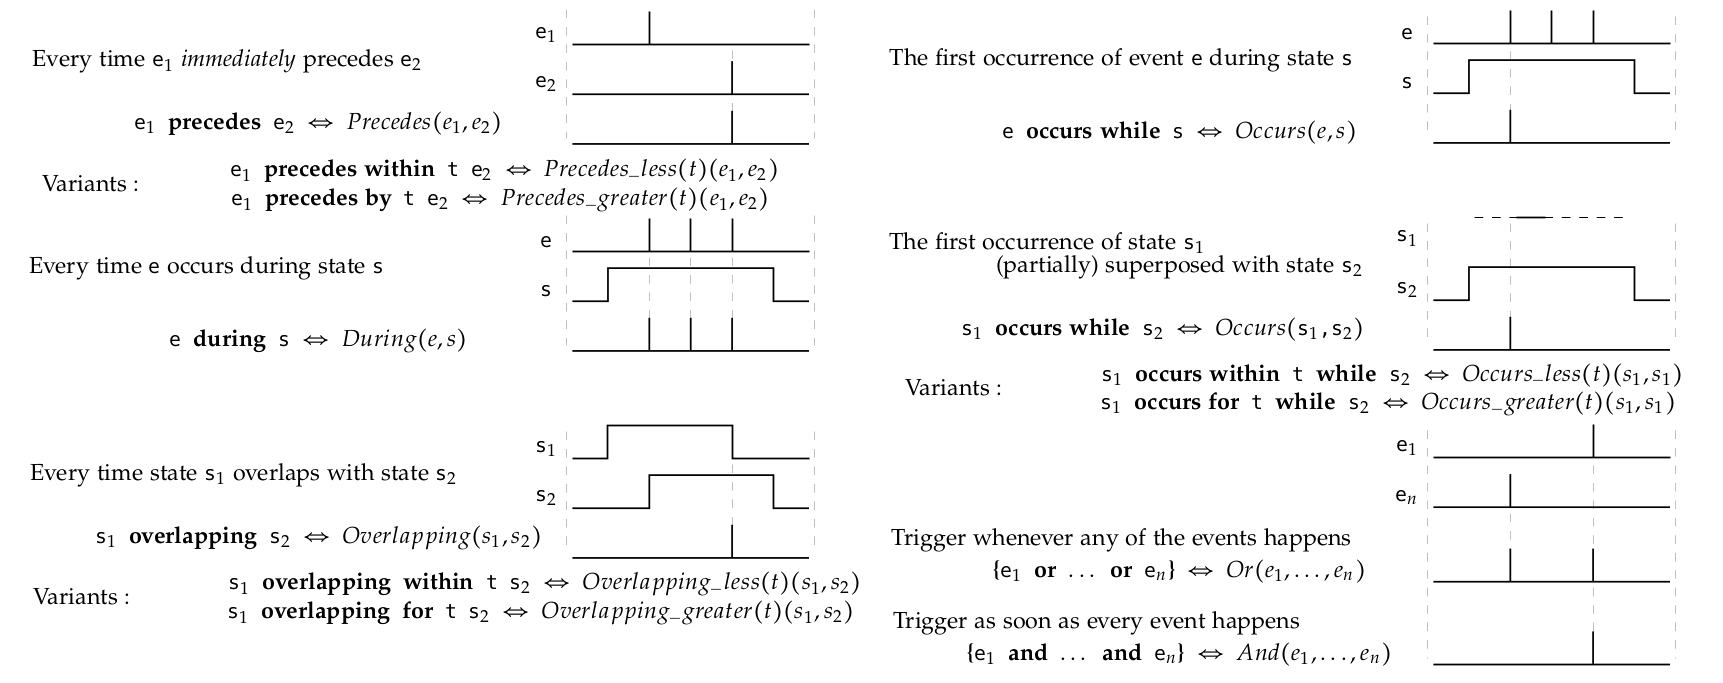
\includegraphics[scale=0.23]{operators.png}
  \end{figure}
\end{frame}
\begin{frame}[fragile]{Opérateurs}
  \addtocounter{framenumber}{-1}
  \begin{figure}[!h]
    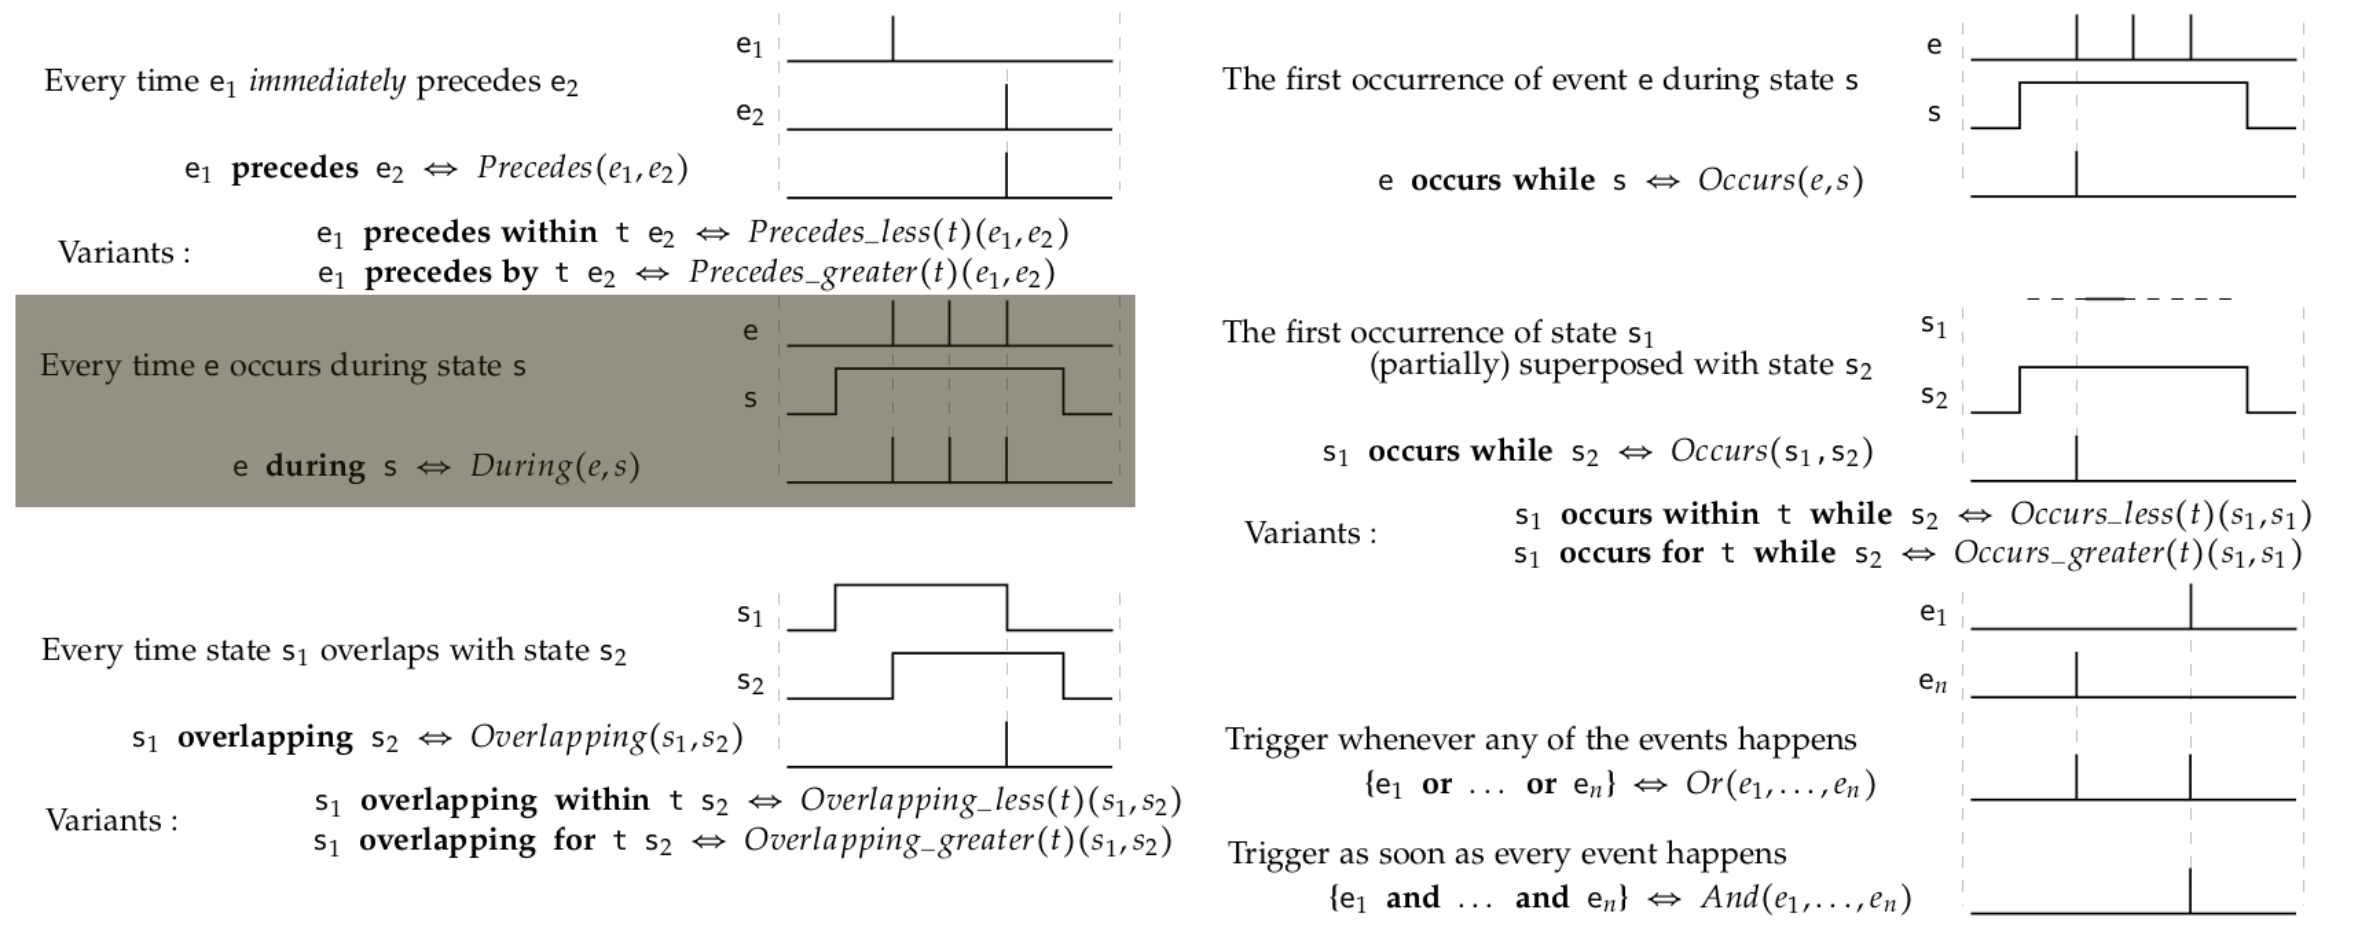
\includegraphics[scale=0.23]{operators_1.png}
  \end{figure}
\end{frame}
\begin{frame}[fragile]{Opérateurs}
  \addtocounter{framenumber}{-1}
  \begin{figure}[!h]
    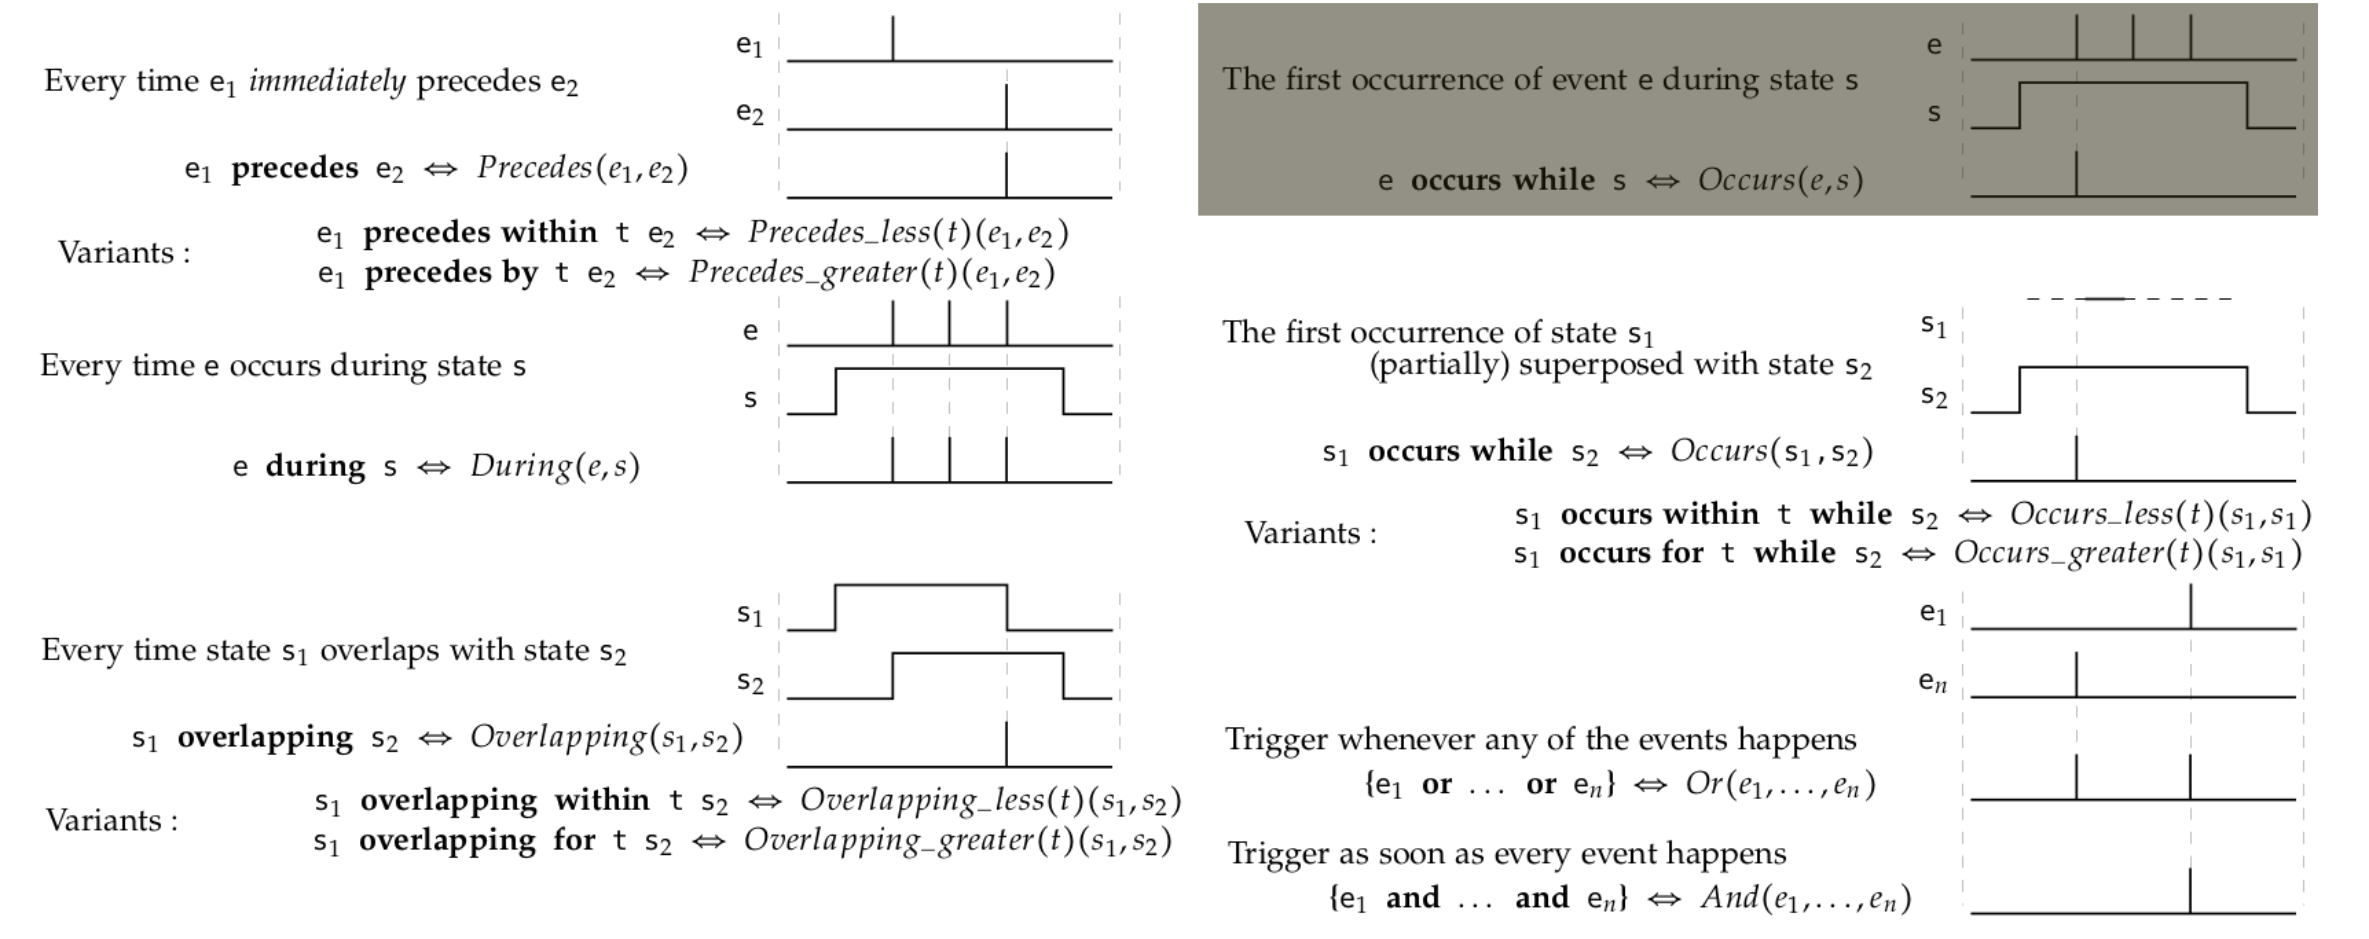
\includegraphics[scale=0.23]{operators_2.png}
  \end{figure}
\end{frame}
\begin{frame}[fragile]{Opérateurs}
  \addtocounter{framenumber}{-1}
  \begin{figure}[!h]
    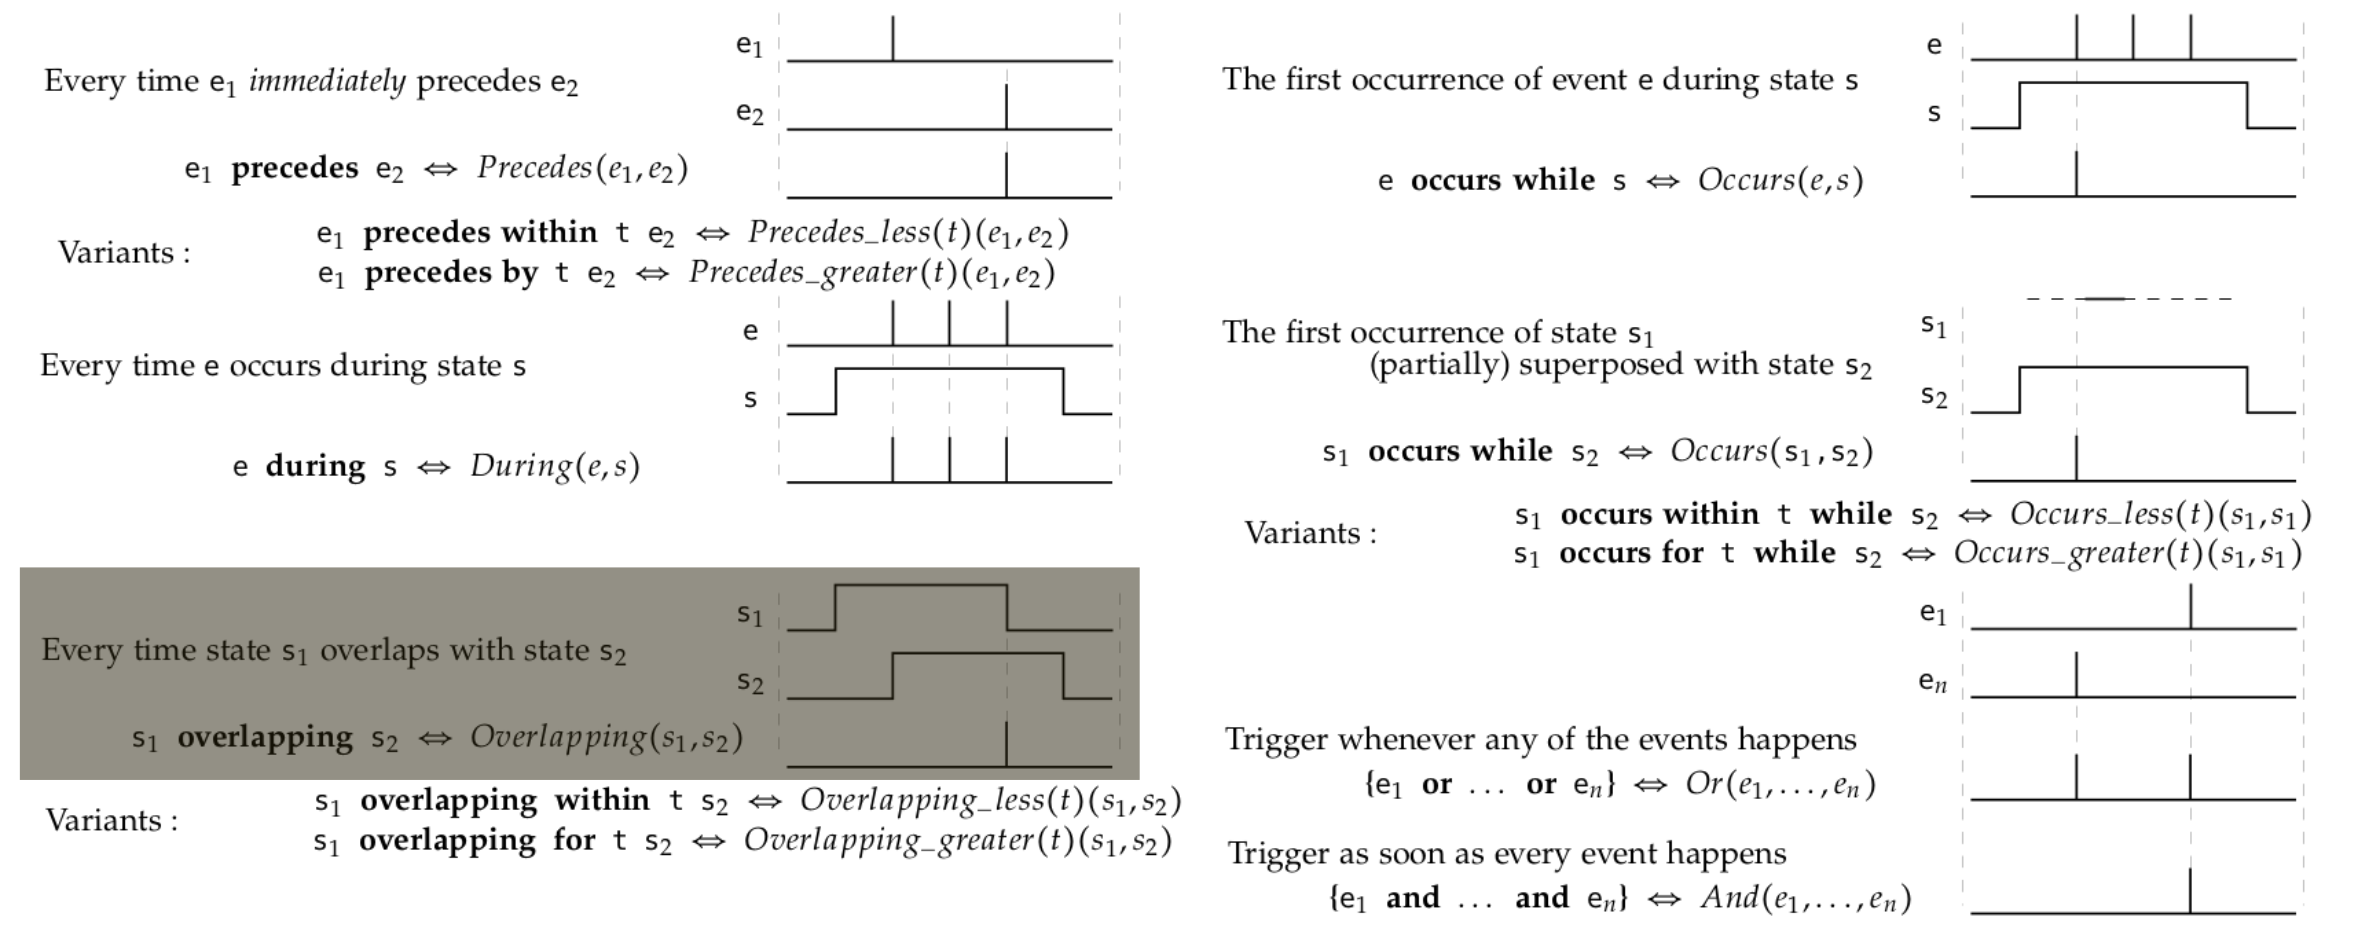
\includegraphics[scale=0.23]{operators_3.png}
  \end{figure}
\end{frame}

% \begin{frame}[fragile]{Définition d'un service}
%   \begin{coloredbox}[gray]{Syntaxe textuelle}
%   \begin{figure}[h]
%     \begin{lstlisting}[language=MaloyaText]
%       { ( freezer becomes open precedes 
%         within 10 minutes stove becomes on )
%         or
%         ( freezer becomes open occurs while stove is on ) 
%       } occurs while lunchTime
%     \end{lstlisting}
%     % \caption{Code Maloya textuel pour le service ``Lunch Reheat''.}
%     \label{listing:maloyaText_reheat} 
%   \end{figure}
% \end{coloredbox}
%  \begin{coloredbox}[gray]{Syntaxe abstraite}
%   \begin{figure}[!h]
%     \begin{lstlisting}[language=Maloya]
%       Occurs(Or(
%         Precedes_less(10min)(freezer => open, stove => on),
%         Occurs(freezer => open, stove = on)),
%       lunchTime)
%     \end{lstlisting}
%     %\caption{Code Maloya interne pour le service ``Lunch Reheat''.}
%     \label{listing:maloya_reheat}
%   \end{figure}
% \end{coloredbox}
% \end{frame}

\begin{frame}[fragile]{Définition d'un service}
  \begin{coloredbox}[black]{Syntaxe textuelle}
  \begin{figure}[h]
    \begin{lstlisting}[language=MaloyaText,basicstyle=\ttfamily\footnotesize,escapechar=!]
      { ( !\colorbox{black!5}{freezer becomes open}! !\colorbox{black!5}{precedes within 10 minutes}! !\colorbox{black!5}{stove becomes on}! )
        !\colorbox{black!5}{or}!
        ( !\colorbox{black!5}{freezer becomes open}! !\colorbox{black!5}{occurs while}! !\colorbox{black!5}{stove is on}! ) 
      } !\colorbox{black!5}{occurs while}! !\colorbox{black!5}{lunchTime}!
    \end{lstlisting}
    % \caption{Code Maloya textuel pour le service ``Lunch Reheat''.}
  \end{figure}
\end{coloredbox}
 \begin{coloredbox}[black]{Syntaxe abstraite}
  \begin{figure}[!h]
    \begin{lstlisting}[language=Maloya,basicstyle=\ttfamily\footnotesize,escapechar=!]
      !\colorbox{black!5}{Occurs}!( !\colorbox{black!5}{Or}!(
        !\colorbox{black!5}{Precedes\_less(10min)}!( !\colorbox{black!5}{freezer => open}!, !\colorbox{black!5}{stove => on}!),
        !\colorbox{black!5}{Occurs}!( !\colorbox{black!5}{freezer => open}!, !\colorbox{black!5}{stove = on}!)),
      !\colorbox{black!5}{lunchTime}!)
    \end{lstlisting}
    %\caption{Code Maloya interne pour le service ``Lunch Reheat''.}
  \end{figure}
\end{coloredbox}
\end{frame}

\begin{frame}[fragile]{Définition d'un service}
\addtocounter{framenumber}{-1}

  \begin{coloredbox}[black]{Syntaxe textuelle}
  \begin{figure}[h]
    \begin{lstlisting}[language=MaloyaText,basicstyle=\ttfamily\footnotesize,escapechar=!]
      { ( !\colorbox{checked!50}{freezer becomes open}! !\colorbox{black!5}{precedes within 10 minutes}! !\colorbox{checked!50}{stove becomes on}! )
        !\colorbox{black!5}{or}!
        ( !\colorbox{checked!50}{freezer becomes open}! !\colorbox{black!5}{occurs while}! !\colorbox{black!5}{stove is on}! ) 
      } !\colorbox{black!5}{occurs while}! !\colorbox{black!5}{lunchTime}!
    \end{lstlisting}
    % \caption{Code Maloya textuel pour le service ``Lunch Reheat''.}
  \end{figure}
\end{coloredbox}
 \begin{coloredbox}[black]{Syntaxe abstraite}
  \begin{figure}[!h]
    \begin{lstlisting}[language=Maloya,basicstyle=\ttfamily\footnotesize,escapechar=!]
      !\colorbox{black!5}{Occurs}!( !\colorbox{black!5}{Or}!(
        !\colorbox{black!5}{Precedes\_less(10min)}!( !\colorbox{checked!50}{freezer => open}!, !\colorbox{checked!50}{stove => on}!),
        !\colorbox{black!5}{Occurs}!( !\colorbox{checked!50}{freezer => open}!, !\colorbox{black!5}{stove = on}!)),
      !\colorbox{black!5}{lunchTime}!)
    \end{lstlisting}
    %\caption{Code Maloya interne pour le service ``Lunch Reheat''.}
  \end{figure}
\end{coloredbox}
\end{frame}

\begin{frame}[fragile]{Définition d'un service}
\addtocounter{framenumber}{-1}

  \begin{coloredbox}[black]{Syntaxe textuelle}
  \begin{figure}[h]
    \begin{lstlisting}[language=MaloyaText,basicstyle=\ttfamily\footnotesize,escapechar=!]
      { ( !\colorbox{checked!50}{freezer becomes open}! !\colorbox{black!5}{precedes within 10 minutes}! !\colorbox{checked!50}{stove becomes on}! )
        !\colorbox{black!5}{or}!
        ( !\colorbox{checked!50}{freezer becomes open}! !\colorbox{black!5}{occurs while}! !\colorbox{black!50}{stove is on}! ) 
      } !\colorbox{black!5}{occurs while}! !\colorbox{black!50}{lunchTime}!
    \end{lstlisting}
    % \caption{Code Maloya textuel pour le service ``Lunch Reheat''.}
  \end{figure}
\end{coloredbox}
 \begin{coloredbox}[black]{Syntaxe abstraite}
  \begin{figure}[!h]
    \begin{lstlisting}[language=Maloya,basicstyle=\ttfamily\footnotesize,escapechar=!]
      !\colorbox{black!5}{Occurs}!( !\colorbox{black!5}{Or}!(
        !\colorbox{black!5}{Precedes\_less(10min)}!( !\colorbox{checked!50}{freezer => open}!, !\colorbox{checked!50}{stove => on}!),
        !\colorbox{black!5}{Occurs}!( !\colorbox{checked!50}{freezer => open}!, !\colorbox{black!50}{stove = on}!)),
      !\colorbox{black!50}{lunchTime}!)
    \end{lstlisting}
    %\caption{Code Maloya interne pour le service ``Lunch Reheat''.}
  \end{figure}
\end{coloredbox}
\end{frame}

\begin{frame}[fragile]{Définition d'un service}
\addtocounter{framenumber}{-1}

  \begin{coloredbox}[black]{Syntaxe textuelle}
  \begin{figure}[h]
    \begin{lstlisting}[language=MaloyaText,basicstyle=\ttfamily\footnotesize,escapechar=!]
      { ( !\colorbox{checked!50}{freezer becomes open}! !\colorbox{teal!50}{precedes within 10 minutes}! !\colorbox{checked!50}{stove becomes on}! )
        !\colorbox{teal!50}{or}!
        ( !\colorbox{checked!50}{freezer becomes open}! !\colorbox{teal!50}{occurs while}! !\colorbox{black!50}{stove is on}! ) 
      } !\colorbox{teal!50}{occurs while}! !\colorbox{black!50}{lunchTime}!
    \end{lstlisting}
    % \caption{Code Maloya textuel pour le service ``Lunch Reheat''.}
  \end{figure}
\end{coloredbox}
 \begin{coloredbox}[black]{Syntaxe abstraite}
  \begin{figure}[!h]
    \begin{lstlisting}[language=Maloya,basicstyle=\ttfamily\footnotesize,escapechar=!]
      !\colorbox{teal!50}{Occurs}!( !\colorbox{teal!50}{Or}!(
        !\colorbox{teal!50}{Precedes\_less(10min)}!( !\colorbox{checked!50}{freezer => open}!, !\colorbox{checked!50}{stove => on}!),
        !\colorbox{teal!50}{Occurs}!( !\colorbox{checked!50}{freezer => open}!, !\colorbox{black!50}{stove = on}!)),
      !\colorbox{black!50}{lunchTime}!)
    \end{lstlisting}
    %\caption{Code Maloya interne pour le service ``Lunch Reheat''.}
  \end{figure}
\end{coloredbox}
\end{frame}


\begin{frame}[fragile]{Étapes de compilation}
  \begin{minipage}{.45\linewidth}
    %\begin{minipage}[t]{.6\linewidth}
      \vspace*{-34.28mm}
      \begin{coloredbox}[black]{\tiny Syntaxe abstraite~:}
      \begin{lstlisting}[language=Maloya,basicstyle=\ttfamily\tiny,escapechar=!]
Occurs(!\colorbox{black!5}{Precedes}!_!\colorbox{black!5}{{\bf less(}10min{\bf )}}!(freezer=>open,
                                !\colorbox{black!5}{stove=>on}!),
       !\colorbox{black!5}{lunchTime}!)
     \end{lstlisting}
\end{coloredbox}
   %\end{minipage}
   \vfill
   %\begin{minipage}[t]{.6\linewidth}
   %\end{minipage}
 \end{minipage}
 \hfill
 \begin{minipage}{.52\linewidth}
   \begin{tiny}
   \end{tiny}
 \end{minipage}
\end{frame}
%*******************************************************************

\begin{frame}[fragile]{Étapes de compilation~: Vers Pseudo-code EPL}
  \begin{minipage}{.45\linewidth}
\vspace*{3.4mm}
    %\begin{minipage}[t]{.6\linewidth}
      \begin{coloredbox}[black]{\tiny Syntaxe abstraite~:}
      \begin{lstlisting}[language=Maloya,basicstyle=\ttfamily\tiny,escapechar=!]
Occurs(!\colorbox{black!5}{Precedes}!_!\colorbox{black!5}{{\bf less(}10min{\bf )}}!(freezer=>open,
                                !\colorbox{black!5}{stove=>on}!),
       !\colorbox{black!5}{lunchTime}!)
     \end{lstlisting}
\end{coloredbox}
   %\end{minipage}
   \vfill
   %\begin{minipage}[t]{.6\linewidth}
            \begin{coloredbox}[black]{\tiny Pseudo-code EPL~:}
     \begin{lstlisting}[language=EPLPseudoCode,basicstyle=\ttfamily\tiny,escapechar=!]
//Window1
( every freezer => open -> !\colorbox{black!5}{stove => on}! 
  and not (freezer=>open)!\colorbox{black!5}{{\bf where timer:within(}10min{\bf )}}!) 

every !\colorbox{black!5}{lunchTime=>begin}! ->
  !\colorbox{black!5}{Window1}!(timestamp > (lunchTime=>begin).timestamp)
  !\colorbox{black!5}{{\bf {\it and not}} lunchTime=>end }!
     \end{lstlisting}
\end{coloredbox}
   %\end{minipage}
 \end{minipage}
 \hfill
 \begin{minipage}{.52\linewidth}
 \end{minipage}
\end{frame}
%*******************************************************************

\begin{frame}[fragile]{Étapes de compilation~: Vers Pseudo-code EPL}
\addtocounter{framenumber}{-1}
\vspace*{3.4mm}
  \begin{minipage}{.45\linewidth}
      \begin{coloredbox}[black]{\tiny Syntaxe abstraite~:}
      \begin{lstlisting}[language=Maloya,basicstyle=\ttfamily\tiny,escapechar=!]
Occurs(!\colorbox{black!5}{Precedes}!_!\colorbox{black!5}{{\bf less(}10min{\bf )}}!(freezer=>open,
                                !\colorbox{black!5}{stove=>on}!),
       !\colorbox{black!50}{lunchTime}!)
      \end{lstlisting}
\end{coloredbox}
    %\end{minipage}
    \vfill
    %\begin{minipage}[t]{.6\linewidth}
            \begin{coloredbox}[black]{\tiny Pseudo-code EPL~:}
      \begin{lstlisting}[language=EPLPseudoCode,basicstyle=\ttfamily\tiny,escapechar=!]
//Window1
( every freezer => open -> !\colorbox{black!5}{stove => on}! 
  and not (freezer=>open)!\colorbox{black!5}{{\bf where timer:within(}10min{\bf )}}!) 

every !\colorbox{black!50}{lunchTime=>begin}! ->
  !\colorbox{black!5}{Window1}!(timestamp > (lunchTime=>begin).timestamp)
  !\colorbox{black!50}{{\bf {\it and not}} lunchTime=>end }!
      \end{lstlisting}
\end{coloredbox}
    %\end{minipage}
  \end{minipage}
  \hfill
  \begin{minipage}{.52\linewidth}
    \vspace*{-69.1mm}
    \begin{tiny}
      \colorbox{black!50}{Gestion des états}
    \end{tiny}
  \end{minipage}
\end{frame}
%*******************************************************************

\begin{frame}[fragile]{Étapes de compilation~: Vers Pseudo-code EPL}
\addtocounter{framenumber}{-1}
\vspace*{3.4mm}
  \begin{minipage}{.45\linewidth}
      \begin{coloredbox}[black]{\tiny Syntaxe abstraite~:}
      \begin{lstlisting}[language=Maloya,basicstyle=\ttfamily\tiny,escapechar=!]
Occurs(!\colorbox{teal!50}{Precedes}!_!\colorbox{black!5}{{\bf less(}10min{\bf )}}!(freezer=>open,
                                !\colorbox{black!5}{stove=>on}!),
       !\colorbox{black!50}{lunchTime}!)
      \end{lstlisting}
\end{coloredbox}
    \vfill
            \begin{coloredbox}[black]{\tiny Pseudo-code EPL~:}
      \begin{lstlisting}[language=EPLPseudoCode,basicstyle=\ttfamily\tiny,escapechar=!]
//Window1
( every freezer => open -> !\colorbox{black!5}{stove => on}! 
  and not (freezer=>open)!\colorbox{black!5}{{\bf where timer:within(}10min{\bf )}}!) 

every !\colorbox{black!50}{lunchTime=>begin}! ->
  !\colorbox{teal!50}{Window1}!(timestamp > (lunchTime=>begin).timestamp)
  !\colorbox{black!50}{{\bf {\it and not}} lunchTime=>end }!
      \end{lstlisting}
\end{coloredbox}
  \end{minipage}
  \hfill
  \begin{minipage}{.52\linewidth}
    \vspace*{-68.7mm}
    \begin{tiny}
      \colorbox{black!50}{Gestion des états},\colorbox{teal!50}{Composition}
    \end{tiny}
  \end{minipage}
\end{frame}
%*******************************************************************

\begin{frame}[fragile]{Étapes de compilation~: Vers Pseudo-code EPL}
\addtocounter{framenumber}{-1}
  \begin{minipage}{.45\linewidth}
    %\begin{minipage}[t]{.6\linewidth}
\vspace*{3.4mm}
      \begin{coloredbox}[black]{\tiny Syntaxe abstraite~:}
      \begin{lstlisting}[language=Maloya,basicstyle=\ttfamily\tiny,escapechar=!]
Occurs(!\colorbox{teal!50}{Precedes}!_!\colorbox{checked!50}{{\bf less(}10min{\bf )}}!(freezer=>open,
                                !\colorbox{black!5}{stove=>on}!),
       !\colorbox{black!50}{lunchTime}!)
      \end{lstlisting}
\end{coloredbox}
    %\end{minipage}
    \vfill
    %\begin{minipage}[t]{.6\linewidth}
            \begin{coloredbox}[black]{\tiny Pseudo-code EPL~:}
      \begin{lstlisting}[language=EPLPseudoCode,basicstyle=\ttfamily\tiny,escapechar=!]
//Window1
( every freezer => open -> !\colorbox{black!5}{stove => on}! 
  and not (freezer=>open)!\colorbox{checked!50}{{\bf where timer:within(}10min{\bf )}}!) 

every !\colorbox{black!50}{lunchTime=>begin}! ->
  !\colorbox{teal!50}{Window1}!(timestamp > (lunchTime=>begin).timestamp)
  !\colorbox{black!50}{{\bf {\it and not}} lunchTime=>end }!
      \end{lstlisting}
\end{coloredbox}
    %\end{minipage}
  \end{minipage}
  \hfill
  \begin{minipage}{.52\linewidth}
    \vspace*{-65.3mm}
    \begin{tiny}
      \colorbox{black!50}{Gestion des états},\colorbox{teal!50}{Composition},\colorbox{checked!50}{Timer explicites}
    \end{tiny}

  \end{minipage}
\end{frame}
%*******************************************************************

\begin{frame}[fragile]{Étapes de compilation~: Vers EPL Esper}
  \begin{minipage}{.45\linewidth}
    %\begin{minipage}[t]{.6\linewidth}
      \begin{coloredbox}[black]{\tiny Syntaxe abstraite~:}

      \begin{lstlisting}[language=Maloya,basicstyle=\ttfamily\tiny,escapechar=!]
Occurs(!\colorbox{teal!50}{Precedes}!_!\colorbox{checked!50}{{\bf less(}10min{\bf )}}!(freezer=>open,
                                !\colorbox{black!5}{stove=>on}!),
       !\colorbox{black!50}{lunchTime}!)
        \end{lstlisting}
\end{coloredbox}
 % \end{minipage}
\vfill
  %\begin{minipage}[t]{.6\linewidth}
        \begin{coloredbox}[black]{\tiny Pseudo-code EPL~:}
      \begin{lstlisting}[language=EPLPseudoCode,basicstyle=\ttfamily\tiny,escapechar=!]
//Window1
( every freezer => open -> !\colorbox{black!5}{stove => on}! 
  and not (freezer=>open)!\colorbox{checked!50}{{\bf where timer:within(}10min{\bf )}}!) 

every !\colorbox{black!50}{lunchTime=>begin}! ->
  !\colorbox{teal!50}{Window1}!(timestamp > (lunchTime=>begin).timestamp)
  !\colorbox{black!50}{{\bf {\it and not}} lunchTime=>end }!
      \end{lstlisting}
\end{coloredbox}
    %\end{minipage}
  \end{minipage}
\hfill
\begin{minipage}{.52\linewidth}
   \begin{tiny}
    \colorbox{black!50}{Gestion des états},\colorbox{teal!50}{Composition},\colorbox{checked!50}{Timer explicites}
  \end{tiny}
  \begin{coloredbox}[black]{\tiny EPL Esper~:}
     \begin{lstlisting}[language=EPL,basicstyle=\ttfamily\tiny,escapechar=|]
create window Wind.std:unique(location,kind,user) 
select * from StreamEvent 

insert into Wind select arg from pattern [ 
  (every arg=StreamEvent(location=`Kitchen',
                         kind=`Freezer',status=`open') ->
     |\colorbox{black!5}{StreamEvent(location=`Kitchen',kind=`Stove',}|
                 |\colorbox{black!5}{status=`on',user=arg.user)}|
     and not (StreamEvent(location=`Kitchen',kind=`Freezer',
                          status=`open',user=arg.user)) 
     where timer:within (10min) ) ]

select Cal_L_b,arg from pattern [ 
  every Cal_L_b= StreamEvent(location=`Lunch',kind=`Calendar',
                             status!=`end') ->
    arg=Wind(timestamp>Cal_L_b.timestamp,user=Cal_L_b.user) 
    and not StreamEvent(location=`Lunch',kind=`Calendar',
                           status=`end',user=Cal_L_b.user) ]
    \end{lstlisting}
\end{coloredbox}
\end{minipage}
\end{frame}
%*******************************************************************
\begin{frame}[fragile]{Étapes de compilation~: Vers EPL Esper}
\addtocounter{framenumber}{-1}
  \begin{minipage}{.45\linewidth}
    %\begin{minipage}[t]{.6\linewidth}
      \begin{coloredbox}[black]{\tiny Syntaxe abstraite~:}
      \begin{lstlisting}[language=Maloya,basicstyle=\ttfamily\tiny,escapechar=!]
Occurs(!\colorbox{teal!50}{Precedes}!_!\colorbox{checked!50}{{\bf less(}10min{\bf )}}!(freezer=>open,
                                !\colorbox{red!30}{stove=>on}!),
       !\colorbox{black!50}{lunchTime}!)
        \end{lstlisting}
      \end{coloredbox}
     % \end{minipage}
      \vfill
      %\begin{minipage}[t]{.6\linewidth}
        \begin{coloredbox}[black]{\tiny Pseudo-code EPL~:}
          \begin{lstlisting}[language=EPLPseudoCode,basicstyle=\ttfamily\tiny,escapechar=!]
//Window1
( every freezer => open -> !\colorbox{red!30}{stove => on}!
  and not (freezer=>open)!\colorbox{checked!50}{{\bf where timer:within(}10min{\bf )}}!) 

every !\colorbox{black!50}{lunchTime=>begin}! ->
  !\colorbox{teal!50}{Window1}!(timestamp > (lunchTime=>begin).timestamp)
  !\colorbox{black!50}{{\bf {\it and not}} lunchTime=>end }!
\end{lstlisting}
\end{coloredbox}
   % \end{minipage}
  \end{minipage}
\hfill
\begin{minipage}{.52\linewidth}
   \begin{tiny}
    \colorbox{black!50}{Gestion des états},\colorbox{teal!50}{Composition},\colorbox{checked!50}{Timer explicites},\colorbox{red!30}{évènements}
  \end{tiny}
  \begin{coloredbox}[black]{\tiny EPL Esper~:}
   \begin{lstlisting}[language=EPL,basicstyle=\ttfamily\tiny,escapechar=|]
create window Wind.std:unique(location,kind,user) 
select * from StreamEvent 

insert into Wind select arg from pattern [ 
  (every arg=StreamEvent(location=`Kitchen',
                         kind=`Freezer',status=`open') ->
     |\colorbox{red!30}{StreamEvent(location=`Kitchen',kind=`Stove',}|
                 |\colorbox{red!30}{status=`on',user=arg.user)}|
     and not (StreamEvent(location=`Kitchen',kind=`Freezer',
                          status=`open',user=arg.user)) 
     where timer:within (10min) ) ]

select Cal_L_b,arg from pattern [ 
  every Cal_L_b= StreamEvent(location=`Lunch',kind=`Calendar',
                             status!=`end') ->
    arg=Wind(timestamp>Cal_L_b.timestamp,user=Cal_L_b.user) 
    and not StreamEvent(location=`Lunch',kind=`Calendar',
                           status=`end',user=Cal_L_b.user) ]
    \end{lstlisting}
\end{coloredbox}
  \end{minipage}
\end{frame}
%*******************************************************************

% \begin{frame}[fragile]{Étapes de compilation}
%   \begin{minipage}[t]{.45\linewidth}
%     \begin{minipage}[t]{.6\linewidth}
%       \begin{lstlisting}[language=Maloya,basicstyle=\ttfamily\tiny,escapechar=!]
% Occurs(Precedes_!\colorbox{checked!50}{{\bf less(}10min{\bf )}}!(freezer=>open,stove=>on),
%        !\colorbox{black!50}{lunchTime}!)
%         \end{lstlisting}
%   \end{minipage}
% \vfill
%   \begin{minipage}[t]{.6\linewidth}
%       \begin{lstlisting}[language=EPLPseudoCode,basicstyle=\ttfamily\tiny,escapechar=!]
% //Window1
% ( every freezer => open -> stove => on 
%     and not (freezer=>open)!\colorbox{checked!50}{{\bf where timer:within(}10min{\bf )}}!) 

% every !\colorbox{black!50}{lunchTime=>begin ->}!
%   !\colorbox{teal!50}{Window1}!( timestamp > (lunchTime=>begin).timestamp )
%   !\colorbox{black!50}{{\bf {\it and not}} lunchTime=>end }!
%       \end{lstlisting}
%     \end{minipage}
%     \begin{minipage}[t]{.6\linewidth}
%       \begin{tiny}
%         \colorbox{black!50}{Gestion des états},\colorbox{checked!50}{Timer explicites},\colorbox{teal!50}{Composition}
%       \end{tiny}
%     \end{minipage}
%   \end{minipage}
% \hfill
%  \begin{minipage}[t]{.45\linewidth}
%    \begin{lstlisting}[language=EPL,basicstyle=\ttfamily\tiny]
% create window Wind.std:unique(location,kind,user) 
% select * from StreamEvent 

% insert into Wind select arg from pattern [ 
%   (every arg=StreamEvent(location='Kitchen',
%                          kind='Freezer',status='open') ->
%      StreamEvent(location='Kitchen',kind='Stove',
%                  status='on',user=arg.user) 
%      and not (StreamEvent(location='Kitchen',kind='Freezer',
%                           status='open',user=arg.user)) 
%      where timer:within (10min) ) ]

% select Cal_L_b,arg from pattern [ 
%   every Cal_L_b= StreamEvent(location='Lunch',kind='Calendar',
%                              status!='end') ->
%     arg=Wind(timestamp>Cal_L_b.timestamp,user=Cal_L_b.user) 
%     and not StreamEvent(location='Lunch',kind='Calendar',
%                         status='end',user=Cal_L_b.user)) ]
% \end{lstlisting}
%  \end{minipage}
% \end{frame}






\begin{frame}{Validation avec le projet Domassist}
\begin{minipage}{.45\linewidth}
\onslide<1->{
\begin{coloredbox}[black]{Expressivité}
Redéfinition de 55 services.
\end{coloredbox}
}
\vfill
\onslide<3->{
\begin{coloredbox}[black]{Performance}
Latence inférieure à une seconde.\\
Occupation mémoire de 352Mo en moyenne. \\
55 règles, 129 installations, H24, 1 mois
% response time of all our rules were always less than a second.\\
% 352MB memory occupancy  (55 rules, data from 129 homes, running 24/7 for one month).
\end{coloredbox}
}
\end{minipage}
\hfill
\begin{minipage}{.45\linewidth}
\onslide<2->{
\begin{coloredbox}[black]{Exactitude}
%Résultats vérifiés avec des scripts Perl simulant les services (55 règles, 129 installations, H24, 1 mois).

\includegraphics[scale=0.225]{perl.png}
\end{coloredbox}
}
\end{minipage}
\vfill
\end{frame}

% \begin{frame}{Synthèse}
%   \begin{itemize}
%   \item Approche unifiée de définition de services.
%   \item Règles manipulant des données de contextes à travers des évènement et des états.
%   \item Abstraction masquant la complexité du traitement d'évènements complexes.
%   \item Réactivité suffisante pour les besoins du domaine.
%   \end{itemize}
% % Unified approach to define services\\
% % Rules manipulating context data as state and event (cover domain concepts).\\
% % Abstraction hides event processing complexity (ease services expression).\\
% % Reactivity sufficient to cover domain requirements.\\
% \end{frame}
